For the following feedback control system, we wish to decrease the effect of the disturbance on the output $y(t)$ by varying $K$. 
\begin{center}
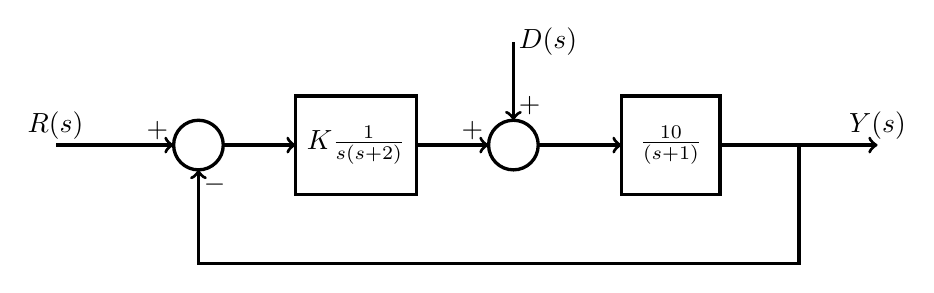
\begin{tikzpicture}[scale=1,inner sep=0pt,outer sep=0pt,very thick,
sysblock/.style={draw,rectangle,inner sep=4pt,minimum width=1.25cm,minimum height=1.25cm,very thick}]

\draw (-2,0) node[draw,circle] (sum1) {$\rule{0pt}{18pt}$};
\draw (0,0) node[sysblock] (K)  {$K\frac{1}{s(s+2)}$};
\draw (2,0) node[draw,circle] (sum2) {$\rule{0pt}{18pt}$};
\draw (4,0) node[sysblock] (G) {$\frac{10}{(s+1)}$};
\draw[<-] (sum1.180) node[above left=2pt] {$+$} -- ++(-1.5,0) node[above=2pt] {$R(s)$};
\draw[->] (sum1.0) -- (K.180);
\draw[->] (K.0) -- (sum2.180) node[above left=2pt] {$+$};
\draw[<-] (sum2.90) node[above right=2pt] {$+$} -- ++(0,1) node[right=2pt] {$D(s)$}; 
\draw[->] (sum2.0) -- (G.180);
\draw[->] (G.0) --  ++(2,0) node[above=2pt] {$Y(s)$};
\draw[->] (G.0) -- ++(1,0) -- ++(0,-1.5) -| (sum1.-90) node[below right=2pt] {$-$};
\end{tikzpicture}
\end{center}
\begin{enumerate}[(a)]
\item What choice of $K$ results in the smallest possible effect on $y(t)$ due to a ramp disturbance?  Hint: the feedback system must be stable.
\item What is the steady state error due to a ramp disturbance for your choice of $K$ in part (a)?
\end{enumerate}

